\documentclass[a4paper, twocolumn]{article}

\usepackage{amsmath}
\usepackage{draftwatermark}
\usepackage{fullpage}
\usepackage[hidelinks]{hyperref}
\usepackage[UKenglish]{isodate}
\usepackage{pgf-pie}
\usepackage{tcolorbox}
\usepackage{url}

\tcbset{height=0.9cm, width=0.8cm, valign=center, halign=center, left=0cm, right=0cm, colback=white}
\newcommand\card[1]{\begin{tcolorbox}#1\end{tcolorbox}}
\newcommand\emphcard[1]{\begin{tcolorbox}[colback=red!30]#1\end{tcolorbox}}

\newcommand\customboard[8]{
  \setlength{\tabcolsep}{0.1cm}
  \begin{tabular}{c c c c}
    #1 & #2 & #3 & #4 \\
    #5 & #6 & #7 & #8 \\
    \customboardmore
}
\newcommand\customboardmore[8]{
    #1 & #2 & #3 & #4 \\
    #5 & #6 & #7 & #8
  \end{tabular}
}
\newcommand\board[8]{
  \setlength{\tabcolsep}{0.1cm}
  \begin{tabular}{c c c c}
    \card{#1} & \card{#2} & \card{#3} & \card{#4} \\
    \card{#5} & \card{#6} & \card{#7} & \card{#8} \\
    \boardmore
}
\newcommand\boardmore[8]{
    \card{#1} & \card{#2} & \card{#3} & \card{#4} \\
    \card{#5} & \card{#6} & \card{#7} & \card{#8}
  \end{tabular}
}

\title{Collapsi is strongly solved}
\author{Michael Young\\University of St Andrews}

\begin{document}

\maketitle

\abstract{ Collapsi is a two-player game of complete information released in
  June 2025 by Mark~S.~Ball of \emph{Riffle Shuffle \& Roll}. Played with two
  pawns on a torroidal board of 16 randomly mixed playing cards, players take it
  in turns to move based on the value of the card they sit on, with the game
  ending when a player has no legal moves.

  The number of possible deals after symmetry breaking is low enough, and the
  game tree shallow enough, to make an exhaustive analysis of the game
  feasible. A solver was written that can find an optimal move for a given board
  position in around 20 milliseconds. A search was applied revealing that the
  first player can force a win in 37.5\% of deals, with the second player able to
  force a win in all others. In 6.4\% of deals the losing player can prolong
  the game to the maximum length of 14 plies; a win can never be forced in
  fewer than 7 plies.
}


\section{The game}

The rules for Collapsi are hosted by the designer in an online document
\cite{rules} and in the game's introductory video \cite{youtube}. The
board is a set of 16 playing cards taken from a standard deck -- four aces, four
2s, four 3s, two 4s and two jokers -- shuffled and arranged into a $4\times 4$
grid, an example layout being shown in Figure \ref{fig:board}. Each player takes
a pawn (red or blue) and places it on a joker, then players take turns
(\textit{plies}) to move with red going first.

\begin{figure}[ht]
  \centering
  \board A223 4A2J 3A23 J3A4
  \caption{Example Collapsi board layout}
  \label{fig:board}
\end{figure}

On a player's first turn they are on a joker, and may choose to move 1, 2, 3 or 4 spaces; on
subsequent turns they must move exactly the number of spaces shown on the card
they begin from, with ace representing 1. Moving is done orthogonally and the
grid is torroidal so that the top edge is joined to the bottom, and the left to
the right. On a given move, a pawn may not enter a given space twice, and may
not end its movement on the space occupied by the opponent's pawn.

After a player's ply, the card they began from is turned face down and cannot
be entered for the rest of the game. The first player who cannot make a legal
move loses the game, which must therefore happen in at most 14 plies.

This study considers which player wins in various layouts given perfect play.


\section{Game length}

In analysing games, besides just considering which player has a winning
strategy, it is common to evaluate how many moves are required to complete the
game assuming perfect play on both sides, as when computing endgame tablebases
such as those for chess \cite{endgame}.

For Collapsi we consider play where the winning player attempts to win in as few
plies as possible, and the losing player attempts to prolong the game, ideally
to the maximum game length of 14 plies. We refer to this as
\textit{game-length-perfect play}. We can evaluate an end-of-game position to
the number of cards remaining face-up if red wins, and the negative of this
number if blue wins -- this is a function that the red player is trying to
maximise, and the blue player is trying to minimise.


\section{Search space}
\label{sec:search-space}

To find a solution, all possible arrangements of the 16 cards must be
considered, naively a space of $16! = 2.1 \times 10^{13}$ possible
arrangements. However, various symmetries allow us to reduce this search space by
eliminating deals that are strategically equivalent, resulting in a more tractable
number of deals that need to be considered.

First observe that suit plays no part in the game: all 3s are equivalent, and so
on. Note also that a player's start position has no effect, since a move of 1. 2. 3 or 4
allows them to reach any uncovered space on their first ply; this means the two
jokers can be considered equivalent.

The torroidal nature of the board means that the bottom row can be moved to the
top, or the right column moved to the left edge, without materially affecting
play. Each of these operations can be cycled, so that any row can be chosen as
the top one and any column as the left one. We exploit this by only considering
boards with a joker in the top-left corner, without loss of generality.

We can also constrain the position of the second joker without loss of
generality, to take advantage of reflections in the board. There are 15 possible positions for the second joker, but two
such positions are strategically equivalent if they have the same $(x, y)$
distance between the first joker and the second,
possibly including an $x$--$y$ swap (diagonal reflection). The possible distances are shown in
Figure~\ref{fig:joker-distances}, with one representative of each distance
highlighted: these 5 positions are the positions considered for the second joker
when searching.

\begin{figure}[ht]
  \centering
  \customboard
  {\card{J}} {\emphcard{0,1}} {\emphcard{0,2}} {\card{0,1}}
  {\card{0,1}} {\emphcard{1,1}} {\emphcard{1,2}} {\card{1,1}}
  {\card{0,2}} {\card{1,2}} {\emphcard{2,2}} {\card{1,2}}
  {\card{0,1}} {\card{1,1}} {\card{1,2}} {\card{1,1}}
  \caption{Distances of spaces from top-left joker}
  \label{fig:joker-distances}
\end{figure}

Though these 5 positions cover all possible deals, they are not equally
likely. As Figure~\ref{fig:joker-distances} shows, of the 15 positions for the
second joker: $(0,1)$, $(1,1)$ and $(1,2)$ represent four each; $(0,2)$
represents two; and $(2,2)$ represents only one. Analysis of statistics for all
possible deals should therefore weight these positions accordingly.

Overall, with the position of one joker fixed, 5 options for the second joker,
and the remaining 14 cards split into three sets of four with the two 4s left
over, the number of deals that must be considered is equal to
$$5~\binom{14}{4} \binom{10}{4} \binom{6}{4} = 15~765~750,$$
a number much more amenable to search than the naive space initially considered.
After weighting the second joker positions as described above, we can produce
data for a total of 47~297~250 deals, which correspond proportionally to a
uniformly random deal.

Different deals have game trees of different sizes, but informal experiments
show that around 900~000 possible games can be played from a typical deal.


\section{Computation}

A Rust library \cite{github} was written that can solve any given game position,
and also enumerate all possible deals as described above. Exhaustive experiments
were performed using a 13th Gen Intel Core i5-13500 processor. All 15~765~750
deals can be enumerated in 3.3 seconds and then explored and solved in
parallel.

The algorithm used for evaluating game positions was minimax search with
alpha--beta pruning and unlimited depth. This was applied both for the simple
goal of finding a winning move, and for the stricter goal of optimising score
with respect to game length.

Given a particular board, it can be determined whether the current player is in
a winning position, and if so a winning move can be determined, in around 12
milliseconds. To find a game-length-perfect move takes slightly longer, around
18 milliseconds. This algorithm is applicable to any game state including those
reached after suboptimal moves have been played, thus satisfying the definition
of a \textit{strongly solved} game \cite{games-solved}. These very short
computation times suggest that there would be little value in the creation of a
database of game positions, since the results can be computed on demand for most
relevant applications.

The result with game-length-perfect play was determined for all deals in a
search that took 7 hours and 29 minutes using 20 cores. All results can be
reproduced by following the instructions provided in the solver's readme file
\cite{github}.


\section{Results}

The length of games given game-length-perfect play from both sides is shown in
Table~\ref{tab:game-length}. Since red plays first, red wins games with an odd
number of plies and blue with an even number of plies.

\begin{table}[ht]
  \centering
  \begin{tabular}{r r r c}
    \hline
    \textbf{Plies} & \textbf{Deals} & \textbf{(\%)} \\
    \hline
    $\leq 6$ & 0 & 0.0 \\
    7 & 24 & 0.0 \\
    8 & 142~686 & 0.3 \\
    9 & 87~936 & 0.2 \\
    10 & 3~238~032 & 6.8 \\
    11 & 5~505~996 & 11.6 \\
    12 & 23~147~802 & 48.9 \\
    13 & 12~127~044 & 25.6 \\
    14 & 3~047~730 & 6.4 \\
    \hline
  \end{tabular}
  \caption{Length of game with perfect play}
  \label{tab:game-length}
\end{table}

A win can never be forced in as few as 6 plies, and there are only 24 positions
(8 up to symmetry) in which red can force a win in the minimum 7 plies, of which
one is shown in Figure~\ref{fig:win-in-7}.

\begin{figure}[ht]
  \centering
  \board JA2A 3JA4 2323 34A2
  \caption{A deal where red wins in 7 plies}
  \label{fig:win-in-7}
\end{figure}

Overall, 17~721~000 deals (37.5\%) are a winning position for red, with the remaining
29~576~250 (62.5\%) a winning position for blue, a considerable advantage for the second
player, as shown in Figure~\ref{fig:win-chance}.

\begin{figure}[ht]
  \centering
  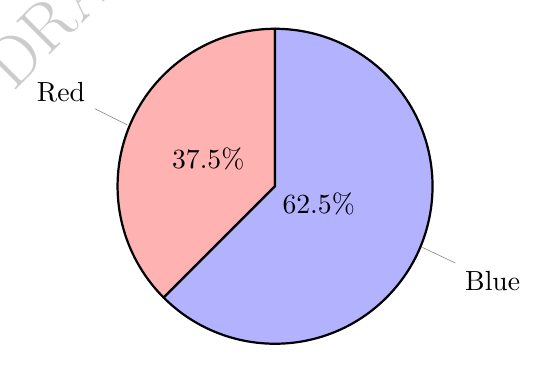
\begin{tikzpicture}
    \pie[
    radius=2,
    color={red!30, blue!30},
    rotate=90,
    text=pin
    ]{
      37.5/Red,
      62.5/Blue
    }
  \end{tikzpicture}
  \caption{Deals won by each player}
  \label{fig:win-chance}
\end{figure}


\section{Future work}

In late June 2025, Collapsi's designer offered an updated set of rules for the
game, described as version 1.2.0, with minor modifications to the rules for movement from
jokers. The solver should be expanded to allow for analysis of the new game,
which may differ in its theoretical status.

The game exploration above was performed exhaustively without consideration for how
this solution could inform human play. Now that a solver exists and perfect
moves can be retrieved easily, its moves should be considered qualitatively,
since they might highlight strategies that players could follow without deep
analysis to improve their play, especially in the early game where it can be
difficult to understand the value of a move.


\section{Acknowledgements}

Thanks to Prof.~Ian Gent for his research suggestions and comments on an early
version, and to Ben Claydon for some valuable tips on data processing in Rust.


\begin{thebibliography}{9}

\bibitem{rules}
  M.~S.~Ball.
  Collapsi 1.1.0.
  Game rules,
  \textit{BoardGameGeek},
  \url{https://boardgamegeek.com/filepage/301918/collapsi-official-rules},
  %\url{https://docs.google.com/document/d/1MV1vvV1Aq7ikRU7lF8Y7QQD-akH3ybHmk2fKs6p61lE}
  2025.

\bibitem{youtube}
  \textit{Riffle Shuffle \& Roll}.
  How to Play Collapsi: \textsc{new} two player abstract game with playing cards!
  \textit{YouTube},
  \url{https://youtu.be/6vYEHdjlw3g},
  2025.

\bibitem{endgame}
  G.~Haworth.
  Chess Endgame News: 7-man `Syzygy' $DTZ_{50}''$ EGTs.
  \textit{ICGA Journal}. 40(4):372--373,
  2018.
  %doi:10.3233/ICG-190087

\bibitem{github}
  M.~Young.
  Collapsi solver.
  Rust crate,
  \textit{Github},
  \url{https://github.com/mtorpey/collapsi},
  2025.

\bibitem{games-solved}
  H.~Jaap van den Herik, Jos W.~H.~M.~Uiterwijk, and Jack~van~Rijswijck.
  Games solved: Now and in the future.
  \textit{Artificial Intelligence}, 134(1):277--311,
  2002.
  %doi:10.1016/S0004-3702(01)00152-7

\end{thebibliography}

\end{document}